\feladatszam Tervezzen henger alakú konzervdobozt, amely térfogata legalább $16\pi\mbox{ cm}^3$, és a felülete minimális. Tehát $V=x_1\pi x_2\geq16\pi$ és $A=2x_1\pi+2x_1\pi x_2\longrightarrow\min!$

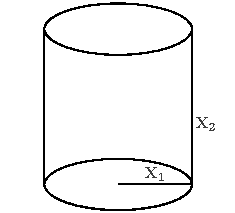
\includegraphics{kepek/kkthenger.pdf}
\end{multicols}

\begin{megoldas}
A KKT feltételek felírásához csoportosítjuk és egyszerűsítjük a feltételeket:
\begin{alignat*}{2}
f&:x_1^2+x_1x_2\\
g_1&:16-x_1^2x_2
\end{alignat*}
\end{megoldas}

\begin{megoldas}
A Lagrange függvény és gradiensei ekkor a következőek:
\begin{gather*}
L(x_1,x_2,u_1)=f+u_1\cdot g_1=x_1^2+x_1x_2+u_1(16-x_1^2x_2)\\
\nabla L=\left(\begin{array}{c}2x_1+x_2-2x_1x_2u_1\\x_1-x_1^2u_1\\\hdashline16-x_1^2x_2\end{array}\right)\quad H=\nabla^2L=\left(\begin{array}{cc:c}2-2x_2u_1&1-2x_1x_2&-2x_1x_2\\1-2x_1x_2&0&-x_1^2\\\hdashline-2x_1x_2&-x_1^2&0\end{array}\right)
\end{gather*}

A KKT feltételek ebből kiolvasva:
\begin{alignat*}{2}
\left.\begin{aligned}
        2x_1+x_2-2x_1x_2u_1&=0\\
        x_1-x_1^2u_1&=0
      \end{aligned}
\right\} &\mbox{ duál feltételek}\\
\left.
        u_1(16-x_1^2x_2)=0
\right.\hskip 0.24cm &\mbox{ komplementaritási feltétel}\\
\left.\begin{aligned}
        16-x_1^2x_2&\leq 0\\
        u_1&\geq 0
      \end{aligned}
\right\} &\mbox{ primál feltételek}
\end{alignat*}

Ezután esetszétválasztással megkeressük az összes KKT pontot:

\textbf{I. eset}: $u_1=0$
\begin{alignat*}{2}
2x_1+x_2&=0\\
x_1&=0\\
16-x_1^2x_2&\leq0
\end{alignat*}

Ebből egyszerűen adódik, hogy $\mathbf{x}=(0,0)^T$, azonban ez nem KKT pont, mert $16\not\leq 0$. Szemléletesen pedig nyilvánvaló hogy egy zérus átmérőjű és magasságú henger térfogata nem lesz megfelelő.

\textbf{II. eset}: $u_1>0$
\begin{alignat*}{2}
2x_1+x_2-2x_1x_2u_1&=0\\
x_1(1-x_1u_1)&=0\\
16-x_1^2x_2&=0
\end{alignat*}

A második feltételnél szétválasztjuk az esetet:

\indent\indent\textbf{II/a. eset}: $x_1=0$. Ekkor $x_2=0$-t kapunk, de azt már beláttuk hogy en nem KKT pont.

\indent\indent\textbf{II/b. eset}: $x_1u_1=1$
\begin{alignat*}{2}
2x_1+x_2-2x_2=&0 \mbox{ azaz } x_2=2x_1\\
16-x_1^2x_2=0
\end{alignat*}
\indent Ebből egyszerűen kijön, hogy
\begin{alignat*}{2}
16&=2x_1^3\\
x_1^3&=8\\
x_1&=2\\
x_2&=4
\end{alignat*}

Az $u_1$ Lagrange szorzó értéke ekkor $\nicefrac{1}{2}$. Az $\mathbf{x}=(2,4)^T$ pont KKT pont, hiszen teljesíti az összes feltételt. Azonban, hogy optimális megoldás legyen teljesülnie kell annak, hogy $H(\textbf{x})$ pozitív definit mátrix legyen.
\end{megoldas}

\begin{megoldas}
A Hesse-féle mátrix értéke az $\mathbf{x}=(2,4)^T$ helyen ($u_1=\nicefrac{1}{2}$):
\begin{gather*}
H(\mathbf{x})=\nabla^2f(\mathbf{x})=\begin{pmatrix}-2&-1&-16\\-1&0&-4\\-16&-4&0\end{pmatrix}
\end{gather*}

Az inerciateszttel ellenőrízhetjük a definitségét:
\begin{gather*}
\underbrace{\left|\begin{array}{ccc}\circled{-2}&-1&-16\\-1&0&-4\\-16&-4&0\end{array}\right|}_\text{Iner(1,0,0)}\sim
\underbrace{\left|\begin{array}{cc}\nicefrac{1}{2}&4\\4&\circled{128}\end{array}\right|}_\text{Iner(0,0,1)}\sim\underbrace{\left|\begin{array}{c}\nicefrac{3}{8}\end{array}\right|}_\text{Iner(0,0,1)}
\end{gather*}

Ez alapján az inercia értéke $\mbox{Iner}(1,0,2)$, tehát H feltételesen pozitív definit mátrix, ezért a $\mathbf{x}=(2,4)^T$ pont valóban optimális minimumpont.
\end{megoldas}
